\chapter{Правило моментов}
{\bfseries Анонс:}\\\\
Плечо силы, момент силы, правило моментов. Вывод передаточного соотношения на силу. Практикум «Весы».\\\\
{\bfseries Цели:}
\begin{itemize}
	\item{}{\bfseries Обучающие:} Повторить основы статики. Освоить практические применения рычагов в механизмах.
	\item{}{\bfseries Развивающая:} Способствовать развитию в учащихся таких качеств как любознательность, усердность, прилежание.\\
\end{itemize}	
{\bfseries Ход занятия:}\\\\
\begin{tabular}[h!]{lll}
	{\hyperlink{lesson20x1}{1. Организационный момент}}&{Презентация}&{(5 мин)}\\
	{\hyperlink{lesson20x2}{2. Рычаги}}&{Презентация}&{(30 мин)}\\
	{\hyperlink{lesson20x3}{3. Передаточное соотношение на силу}}&{Презентация}&{(30 мин)}\\
	{\hyperlink{lesson20x4}{4. «Весы»}}&{Игра}&{(40 мин)}\\
\end{tabular}\\\\

{\hypertarget{lesson20x1}{\blackBlueText{I. Организационный момент}}}\\\\

Первые два раздела занятия представляют собой краткую презентацию перед всей группой. Работа по практикуму «Весы» производится группами по 2 человека. Перед началом работы при необходимости нужно кратко вспомнить основы работы с датчиками и поиск необходимых команд языка в Help.\\\\
\clearpage
{\hypertarget{lesson20x2}{\blackBlueText{II. Рычаги}}}\\\\	

{\slshape Правило рычага по программе относится к курсу физики 7 класса. Однако, как показала практика, легкое повторение является необходимым в группах любого возраста.}

Представим себе один из простейших механизмов, знакомых всем с детских лет~--- качели. Если на них сядут два мальчика~--- тяжелый и легкий, что произойдет? Правильно, тяжелый мальчик перетянет и останется на земле, а легкой будет висеть в воздухе.\\\\

\greenText{Рис}\\\\

Посадим на них близнецов. Оба мальчика окажутся на одном уровне, их вес одинаков. Теперь, допустим хулиганы сломали одно плечо качелей, и оно стало в два раза короче. Что произойдет если теперь посадить двух близнецов на качели?  Казалось бы их вес не изменился, равновесие не должно нарушиться? Однако, опыт показывает что теперь один из братьев перевешивает.\\\\

\greenText{Рис}\\\\

Зато на неисправных качелях легкий мальчик теперь может уравновесить тяжелого.\\\\

\greenText{Рис}\\\\

Многочисленные опыты позволили выяснить, что когда качели в равновесии всегда выполняется следующее:

\begin{equation}
F_1*l_1=F_2*l_2
\end{equation}		

где \(F_1\) и \(F_2\)~--- это силы тяжести мальчиков, а \(l_1\) и \(l_2\)~--- длины половинок качелей.

{\slshape Для классов старше восьмого можно пояснить, что это частный случай общего физического закона: правила моментов. Закон гласит, что твердое тело не вращается, если алгебраическая сумма моментов всех сил, действующих на тело равна нуля.
	
	\begin{equation}
	\sum_i{F_i*l_i}=0
	\end{equation}		
	
	Под «алгебраической» суммой понимается сумма с учетом знаков, т.е. моменты сил вращающих в одну сторону берутся с положительным знаком, а моменты сил вращающих в противоположную сторону~--- с отрицательным. Момент силы равен произведению силы \(F\) на ее плечо \(l\). Плечом силы называется расстояние от оси вращение до линии вдоль которой действует сила.}

\begin{figure}[h!]
	\begin{center}
		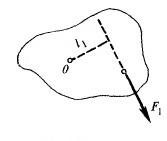
\includegraphics[width=0.3\linewidth]{chapters/chapter20/images/1}
		\caption{\(l\)~--- плечо силы \(F\).}
		\label{ris:image20x1}
	\end{center}
\end{figure}

В обычной жизни люди постоянно сталкиваются с необходимостью учитывать правило моментов. Задумывались ли вы, почему ручка двери расположена не в центре, а как можно дальше от петель на краю? Правильно, так плечо прикладываемой силы получается больше и сила, чтобы открыть дверь требуется меньшая.\\\\

\greenText{Рис двери и изобр плеча на двери}\\\\

Так же можно обсудить с учащимися следующие вопросы:

\begin{enumerate}
	\item Почему у автобусов руль большего диаметра, чем у легковой автомашины?
	\item Как можно приподнять тяжелый груз?
	\item  На рис. изображено строение человеческой руки. Под действием силы двуглавой мышцы (сила F) рычаг-рука поднимает груз в 10 раз превышающий вес шара в руке. Не является ли это «ошибкой природы», свидетельством несовершенства конструкции человека?
	\clearpage
	\begin{figure}[h!]
		\begin{center}
			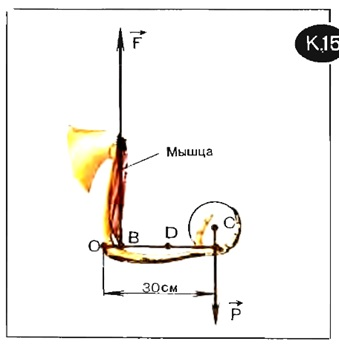
\includegraphics[width=1\linewidth]{chapters/chapter20/images/2}
			\caption{}
			\label{ris:image20x2}
		\end{center}
	\end{figure}	
\end{enumerate}

{\slshape На самом деле такое устройство руки является как раз весьма совершенным.Мы действительно проигрываем в силе, но это оказывается не первостепенным~---мышцы обладают большой силой. Зато мы существенно выигрываем в других отношениях. Небольшое сокращение мышцы позволяет осуществить значительное перемещение ладони с грузом (мы умеем поднимать ее даже до плеча). Кроме этого мы выигрываем в скорости перемещения. Мышцы не могут быстро сокращаться, но при таком рычаге это и не требуется, скорость ладони оказывается в 10 раз больше скорости сокращения.
	
	Если бы мышца была прикреплена к середине лучевой кости D, то мы смогли бы поднимать в 5 раз более тяжелые грузы, но мы бы в 5 раз проиграли в высоте и скорости подъема. Мы сделались бы медленными, неуклюжими и неизящными.}

И конечно,  нельзя не вспомнить известнейшую фразу Архимеда: «Дайте мне точку опоры, и я переверну весь мир». Действительно ли древнегреческому философу не хватило только точки опоры? Под миром, вслед за Архимедом будем понимать всего-то навсего наш земной шар, масса которого \(М=6*10^24\) кг.  Пусть Архимед может поднимать даже 100 кг. Это значит, что плечо рычага за который он будет держаться должно быть в \(6*10^22\) раз длиннее, плеча рычага прикрепленного к Земле. Если от Земли до «точки опоры» 1 метр, то Архимед удалился на \(6*10^19\) км или примерно 6 миллионов световых лет. Т.е. добирался он до этой окраины не меньше 6 млн лет, причем вместе с негнущимся стержнем длиной в \(6*10^19\) км. Но помимо всего этого, есть еще и золотое правило механики:

{\bfseries Во сколько раз выигрываем в силе, во столько раз проигрываем в расстоянии.}

В применении к данному примеру это значит, что даже найдя точку опоры,улетев невозможно далеко, с невозможным рычагом, Архимеду для перемещения Земли на 1 мм понадобиться переместится еще на \(6*10^19\) км.

\begin{figure}[h!]
	\begin{center}
		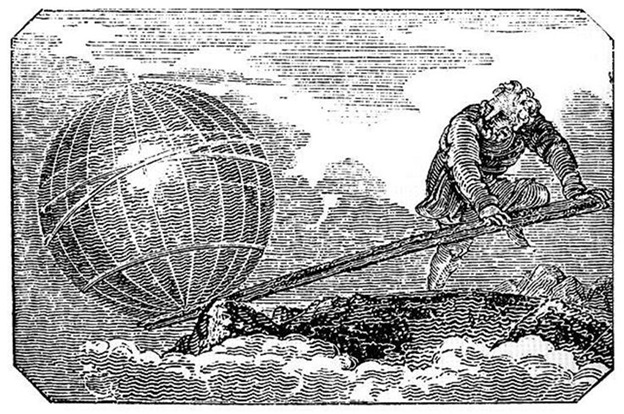
\includegraphics[width=1\linewidth]{chapters/chapter20/images/3}
		\caption{}
		\label{ris:image20x3}
	\end{center}
\end{figure}

{\hypertarget{lesson20x3}{\blackBlueText{III. Передаточное соотношение на силу}}}\\\\

В Занятии \ref{lesson6} было доказано, что при передачи вращения с большей шестеренки на меньшую, происходит выигрыш в скорости. Так же было упомянуто, и активно использовалось впоследствии, что при этом мы во столько же раз проигрываем в силе, но никаких подкрепляющих это рассуждений проведено не было. Теперь мы можем восполнить этот пробел.

\begin{figure}[h!]
	\begin{center}
		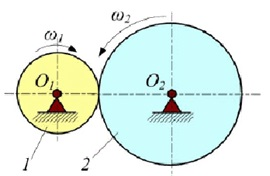
\includegraphics[width=0.45\linewidth]{chapters/chapter20/images/4}
		\caption{}
		\label{ris:image20x4}
	\end{center}
\end{figure}

Шестеренки не проскальзываю, поэтому в точке касания, сила с которой первая шестеренка действует на вторую равна силе, с которой вторая шестеренка действует на первую. При этом силы в оси шестеренки оказываются относящимися как радиусы, а значит и как число зубьев в шестеренках, что обратно передаточному числу.

{\hypertarget{lesson20x4}{\blackBlueText{IV. «Весы»}}}\\\\

\noindent\underline{Задание 1:} Определить порог силы, при которой нажимается копка Touch Sensor.\\
Дан набор разновесов.\\\\

\greenText{Окажется, что кнопка нажимается при весе груза больше 50 граммов.}\\\\

\noindent\underline{Задание 2:} Имеются два абсолютно одинаковых внешне кольца, одно весит 25 г, другое 75 г. Робот имеет корзинку для кольца, при помещении тяжелого кольца в эту корзинку он должен издать звук.

Один из простейших вариантов корзинки  представлен на рис. На дне корзинки укреплен датчик нажатия, который окажется нажат, если положить тяжелое кольцо  и не нажат, если положить легкое кольцо. 

По нажатию кнопки программа проигрывает один из стандартных аудиофайлов.\\\\

{\programm
	{\slshape\bC{if}}\rC{(\bbC{SensorValue}[\rrC{S1}])}\indent\indent\gC{// if the Button is pressed}\\
	\rC{\{}\\
	\indent\bbC{playSound}\rC{(\rrC{soundBeepBeep});}\indent\gC{// play the sound 'soundBeepBeep'}\\
	\rC{\}}\\
}\\\\

\begin{figure}[h!]
	\begin{center}
		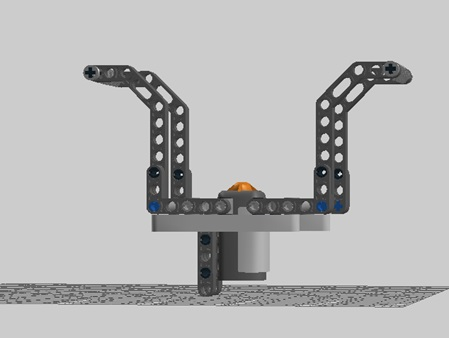
\includegraphics[width=0.8\linewidth]{chapters/chapter20/images/5}
		\caption{}
		\label{ris:image20x5}
	\end{center}
\end{figure}

\begin{figure}[h!]
	\begin{center}
		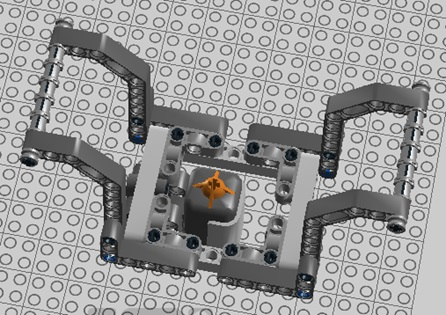
\includegraphics[width=0.8\linewidth]{chapters/chapter20/images/6}
		\caption{}
		\label{ris:image20x6}
	\end{center}
\end{figure}

\noindent\underline{Задание 3:} Имеется два абсолютно одинаковых внешне кольца, одно весит 75 г, другое 210 г. Робот имеет корзинку для кольца, при помещении тяжелого кольца в эту корзинку он должен издать звук.

Понятно, что теперь обе массы больше предела, т.е. при такой же конструкции как в прошлый раз кнопка будет всегда нажата. Однако, если класть груз на одно плечо рычага, которое в 3 раза меньше другого, нажимающего кнопку, то сила действия на кнопку опять будет равна 25 г и 70 г соответственно для легкого и тяжелого колец.\\\\

\greenText{фото конструкции робота в этом случае}